%!TEX program = lualatex
\documentclass[
    paper=letter,
    parskip=half-,
    DIV=10,
    % draft
]{scrartcl}

% WTF? UTF-8 is ignored without this!?? Should be the default on lualatex.
\usepackage[utf8]{luainputenc}

\usepackage{hyperref}
\usepackage{xspace}
\usepackage{mathtools}
\usepackage[final]{microtype}

\usepackage{tikz}
\usetikzlibrary{intersections,calc,arrows,positioning}

\newcommand{\gratio}{\emph{golden ratio}\xspace}

\usepackage{minted}
\usemintedstyle{friendly}

\begin{document}
    \section{Introduction}

    I want to print some of my photos, and to frame them using a simple mat (no framing).

    To do that, I need to choose a border size, and to center it “optically” so the image doesn’t give the impression of sinking into the frame. I also require the top border to be at least as big as the side borders.

    Some people\footnote{\url{http://kombat.org/FrameMaking/step1.html} uses $\phi$ to multiply the longest side and use that border for both sides} use the \emph{golden ratio} ($\phi$) as a multiplicator to the width and height of the size of the mat’s window. I personnally find it produces borders that are way too big.

    Others\footnote{\url{http://www.phimatrix.com/matte-frame-golden-ratio/}} use $\phi$ as a multiplicator to the \emph{area} of the print surface to compute the surface of the mat.

    It gives a size that I like, however it also means the shortest side has smaller borders, which is visually ugly if this happens to be a landscape.

    I could simply use the longest side for all sides, but then I would have other problems:
    \begin{itemize}
        \item “visually centering” the window would still give a smaller top border than the edges,
        \item and on an image with a strong difference between the two dimensions, this could produces borders too big.
    \end{itemize}

    So I decided to:

    \begin{itemize}
        \item use the golden ratio to compute the area of the mat size;
        \item keep the resulting border surface constant;
        \item compute the 4 borders so that the top equals the side borders, and the bottom is bigger accorging to the most common vertical centering rules.
    \end{itemize}

    \section{Optical centering}

    To center the print window on a mat, the most common technique (actually the only one I found aside “move the picture a big higher”) is:

    \begin{enumerate}
        \item align the top left corner of the print with the top left corner of the mat,
        \item draw a vertical line at the center of the remaining space on the right to produce the left and right borders,
        \item draw an horizontal line at the center of the remaining space on the bottom to produce the top and left borders before correction,
        \item draw a line from the bottom left corner of the print to a point placed on the absolute right side of the mat, and the lower left line,
        \item move the picture so the bottom right corner alligns with the diagonal line and the rightmost vertical line.
    \end{enumerate}

    Visually, you get something like the figure \ref{fig:mat}.

    \begin{figure}
    \caption{Centering a print on a mat}\label{fig:mat}
    \centering
    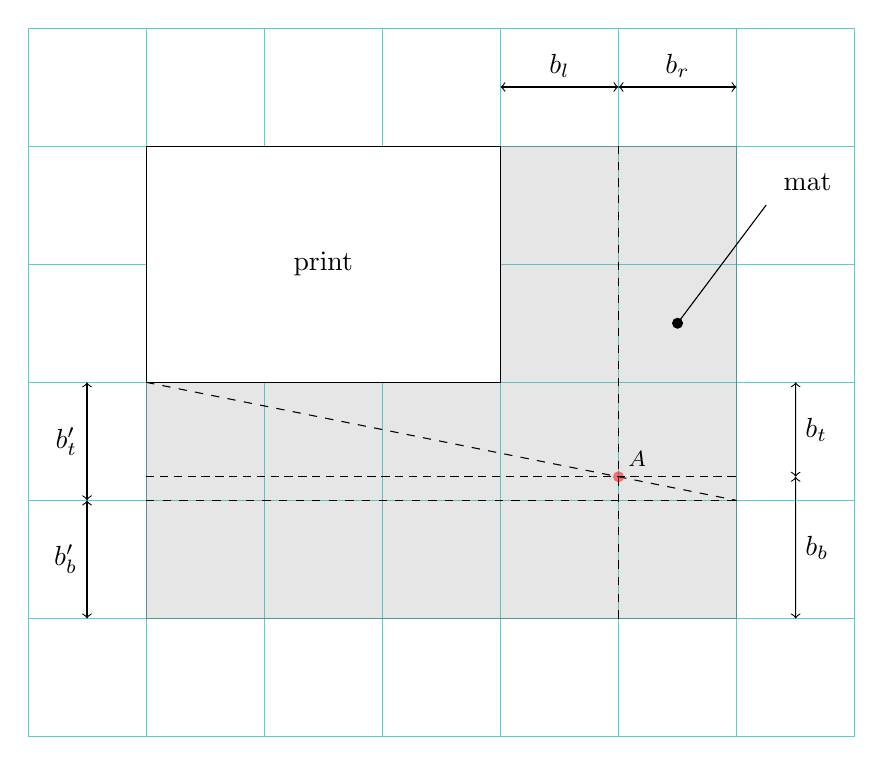
\begin{tikzpicture}[x=1.5cm,y=1.5cm]
        \draw[help lines,very thin,color=blue!50!green!50,step=1] (-1, -1) grid (6, 5);

        % Mat
        \draw[fill=gray,opacity=0.2] (0,4) rectangle +(5,-4);
        % Window
        \draw[fill=white] (0,4) rectangle +(3,-2);
        \node (window) at (1.5,3) {print};

        \draw[-] (4.5,2.5) -- (5.25,3.5);
        \fill[black] (4.5,2.5) circle (2pt);
        \draw (5.6,3.7) node {mat};

        % Border separators
        \draw[dashed,name path=bsepbt] (0,1) -- +(5,0);
        \draw[dashed,name path=bseplr] (4,0) -- +(0,4);

        % diag line and helper line
        \draw[dashed,name path=diag] (0,2) -- (5,1);
        \fill[
            name intersections={of=diag and bseplr,by=I},
            red, opacity=0.5,
            every node/.style={above right, black, opacity=1}
        ]   (I) circle (2pt) node {\footnotesize $A$};
        \coordinate (Ileft) at ($(I) + (-4,0)$);
        \coordinate (Iright) at ($(I) + (1,0)$);
        \draw[
            densely dashed,name path=bsepi,
        ]   (Ileft) -- (Iright);

        % Border arrows
        \begin{scope}[<->,shift={(3,4.5)}]
            \draw (0,0) -- +(1,0) node [above,midway] {$b_l$};
            \draw (1,0) -- +(1,0) node [above,midway] {$b_r$};
        \end{scope}
        \begin{scope}[<->,shift={(-.5,0)}]
            \draw (0,0) -- +(0,1) node [left,midway] {$b'_b$};
            \draw (0,1) -- +(0,1) node [left,midway] {$b'_t$};
        \end{scope}
        \draw[<->] (5.5,0) -- ($(Ileft) + (5.5,0)$) node [right,midway] {$b_b$};
        \draw[<->] ($(Ileft) + (5.5,0)$) -- (5.5,2) node [right,midway] {$b_t$};

        % And an action text..
        % \draw[->] (3,2) -- (I) node [midway,above,right] {\footnotesize move};

    \end{tikzpicture}
    \end{figure}

    On that figure, $b_l$, $b_r$, $b'_t$ and $b'_b$ represent the borders around a perfectly centered print. Normally we want the left and right borders to be the same size, and the top and bottom borders too.

    So we can define $b_x = b_l = b_r$ as the size for the borders along the X axis, and $b_y = b'_t = b'_b$ for the top and bottom borders.

    $b_t$ and $b_b$ represent the top and bottom border of an “optically centered”, obtained by sliding the print so its bottom right corner is set on point $A$. Their value is:

    \begin{align*}
        b_t &= b'_t - A \\
        b_b &= b'_b + A
    \end{align*}

    Let say that $(w_x, w_y)$ are the width and height of the mat’s window (or print size), and $(w_x, w_y)$ the dimensions of the mat itself.

    It can be shown that the amount of upward shift, $A$, is:

    \[
        A = \frac{b_x b_y}{m_x} = \frac{b_x b_y}{w_x + 2b_x}
    \]

    % where $b_x = \frac{m_x - w_x}{2}$ and $b_y = \frac{m_y - w_y}{2}$.

    Personnally, what I want is to find the proper border sizes to that $b_x = b_y = b$, and $b_b = b + A$.


\section{Golden Ratio}

    Let the golden ratio be $\phi$, because I don’t intend on typing “golden ratio” more than I have to.

    What I want is to set the mat’s surface as $\phi w_x w_y$. That means:

    \newcommand{\sphi}{\sqrt{\phi}}
    \begin{align*}
        m_x &= \sphi w_x \\
        m_y &= \sphi w_y
    \end{align*}

\section{Finding the border sizes}

    From a bit of trigonometry, we have
    \begin{align}
        m_x &= w_x + 2b \\
        m_y &= w_y + 2b + A = w_y + 2b + \frac{b^2}{mx - b} \\
        w_x &= m_x - 2b \\
        w_y &= m_y - 2b - A = m_y - 2b - \frac{b^2}{mx + b}
    \end{align}

    The golden ratio of the area gives us:
    \begin{align}
        0 &= \phi w_x w_y - m_x m_y
    \end{align}

    So if we mix those to compute $b$ from the window's dimensions:
    \begin{equation}\label{eq:bwin}
        0 = 6b^3 + (7w_x + 2w_y)b^2 + (2w_x^2 + (3 - \phi)w_xw_y)b + (1 - \phi)w_x^2w_y
    \end{equation}
    And to compute $b$ from the mat's dimensions:
    \begin{equation}\label{eq:bmat}
        % 0 = -2\phi b^3\phi +b^2(5m_x + 2m_y)\phi + b((1 - 3\phi)m_y - 2m_x\phi)m_x + (\phi - 1)m_x^2m_y
        0 = -2\phi b^3 + (5m_x + 2m_y)\phi b^2 + (m_y - 2m_x\phi + 3m_y\phi)m_xb + (\phi - 1)m_x^2m_y
    \end{equation}


\section{Implementing}

Solving symbolically is not really practical, producing way too much complexity for not much.

In the methods presented in table \ref{tbl:times}, the methods producing the best precision should be \texttt{mpmath}, because it's an arbitrary precision library, and \texttt{sympy} because it keeps everything symbolically, and finally evaluates using \texttt{mpmath}.

The least precise method should be \texttt{scipy} because \texttt{fsolve} is very general and doesn't even guarantee a proper result.

The fastest should be \texttt{numpy} because it uses the CPU's floating point.

Table \ref{tbl:times} shows the processing times for a 9x6 print.

Practically, the precision has no impact since any of these methods should produce way more than what I can achieve while cutting a mat sheet. Thus only speed has a meaning in this case.

Pure processing time should point to \texttt{numpy}, however if we account for python’s startup time, \texttt{numpy} takes on average $0.11$s on my computer to run, while \texttt{mpmath} (with and without \texttt{gmpy}) takes $0.06$s.

Thus my final choice is \texttt{mpmath}. It also happens to be much simpler (at least in virtual environments) and faster to install than \texttt{numpy}.

\begin{table}
\caption{Solving times, based on 1000 iterations (except sympy, which is based on 10)}\label{tbl:times}
\centering
\begin{tabular}{llll}
\hline
Library              & time / iteration  & $b$ & $b_b$ \\
\hline
numpy                & $0.000171954$s    & 0.956913776241981   & 1.04887841465701 \\
scipy                & $0.000365011$s    & 0.956913776241981   & 1.04887841465701 \\
mpmath (gmpy)        & $0.003560504$s    & 0.956913776241981   & 1.04887841465701 \\
mpmath               & $0.005906222$s    & 0.956913776241981   & 1.04887841465701 \\
sympy (gmpy)         & $1.134872603$s    & 0.956913776241981   & 1.04887841465701 \\
sympy                & $1.259345698$s    & 0.956913776241981   & 1.04887841465701 \\
\hline
\end{tabular}
\end{table}


\section{Examples}

Using \texttt{mpmath} with the python code from figure \ref{code:solver1}, for a 9x6 print size, we obtain:

    \begin{align*}
        b &= 0.95691 \\
        b_{bot} &= 1.0489
    \end{align*}

\begin{figure}
\label{code:solver1}
\caption{A simple example of numerically solving $b$ from equation \ref{eq:bwin}}
\begin{minted}[mathescape,
               linenos,
               numbersep=5pt,
               frame=lines]{python}
from mpmath import mp

mp.dps = 5

wx = mp.mpf('9'); wy = mp.mpf('6')
phi = (1 + mp.sqrt(5)) / 2
coeffs = [
    6,
    7 * wx + 2 * wy,
    wx * ((3 - phi)*wy + 2*wx),
    (1 - phi) * mp.power(wx, 2) * wy
]

roots = mp.polyroots(coeffs, 15)
b = [root for root in roots if mp.im(root) == mp.mpf(0)][0]
bottom = b + mp.power(b, 2) / (wx + b)

print("Print dimensions: {wx!s} x {wy!s}\n"
      "Resulting border: {b!s}\n"
      "Resulting bottom border: {bottom!s}"
      .format(wx=wx, wy=wy, b=b, bottom=bottom))
\end{minted}
\end{figure}


Assuming the lengths are in centimeters, you can find representation of this at scale in figure \ref{fig:phi}.

If we want to compute the border area so we have the \emph{lengths} (width and height) as $m_{(x|h)} = \phi\cdot w_{(x|h)}$, we use $\phi' = \phi^2$ and obtain the following borders, represented in figure \ref{fig:phisquare}:

\begin{align*}
    b &= 2.1285 \\
    b_{bot} &= 2.5356
\end{align*}

    \begin{figure}
    \caption{Result for a 9x6cm print using $m_a = \phi w_a$}\label{fig:phi}
    \centering
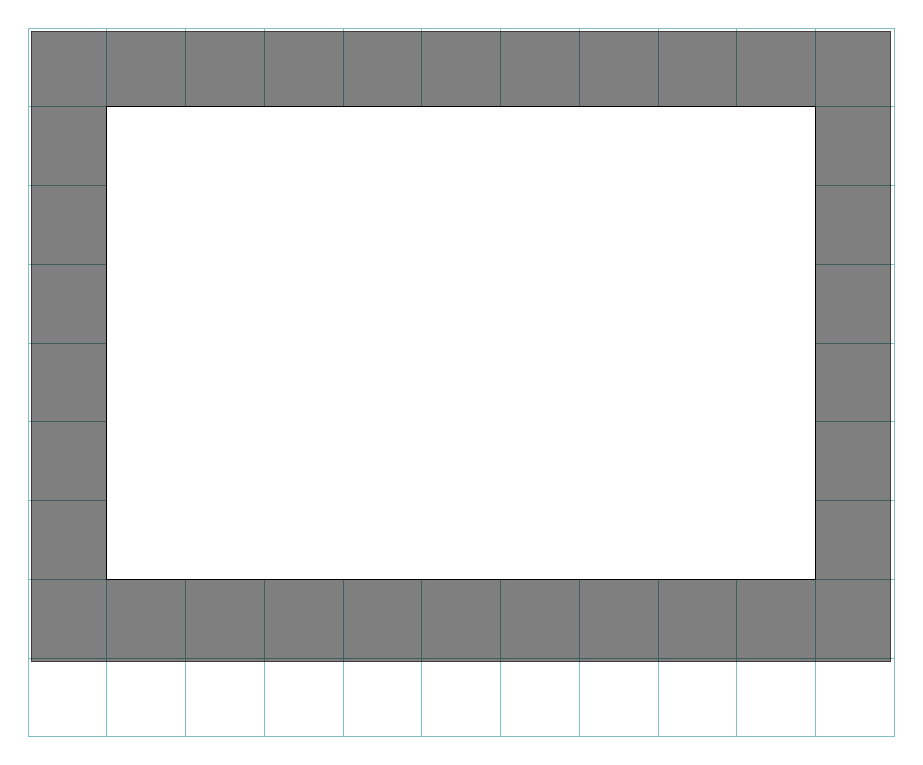
\begin{tikzpicture}
    \draw[help lines,very thin,color=blue!50!green!50,step=1] (-1.0, 1.0) grid +(11.0, -9.0);
    % Mat
    \draw[fill=black,opacity=0.5] (-0.95691,0.95691) rectangle +(10.914,-8.0058);
    % Window
    \draw[fill=white] (0,0) rectangle +(9,-6);
\end{tikzpicture}
    \end{figure}


    \begin{figure}
    \caption{Result for a 9x6cm print using $m_a = \phi^2 w_a$}\label{fig:phisquare}
    \centering
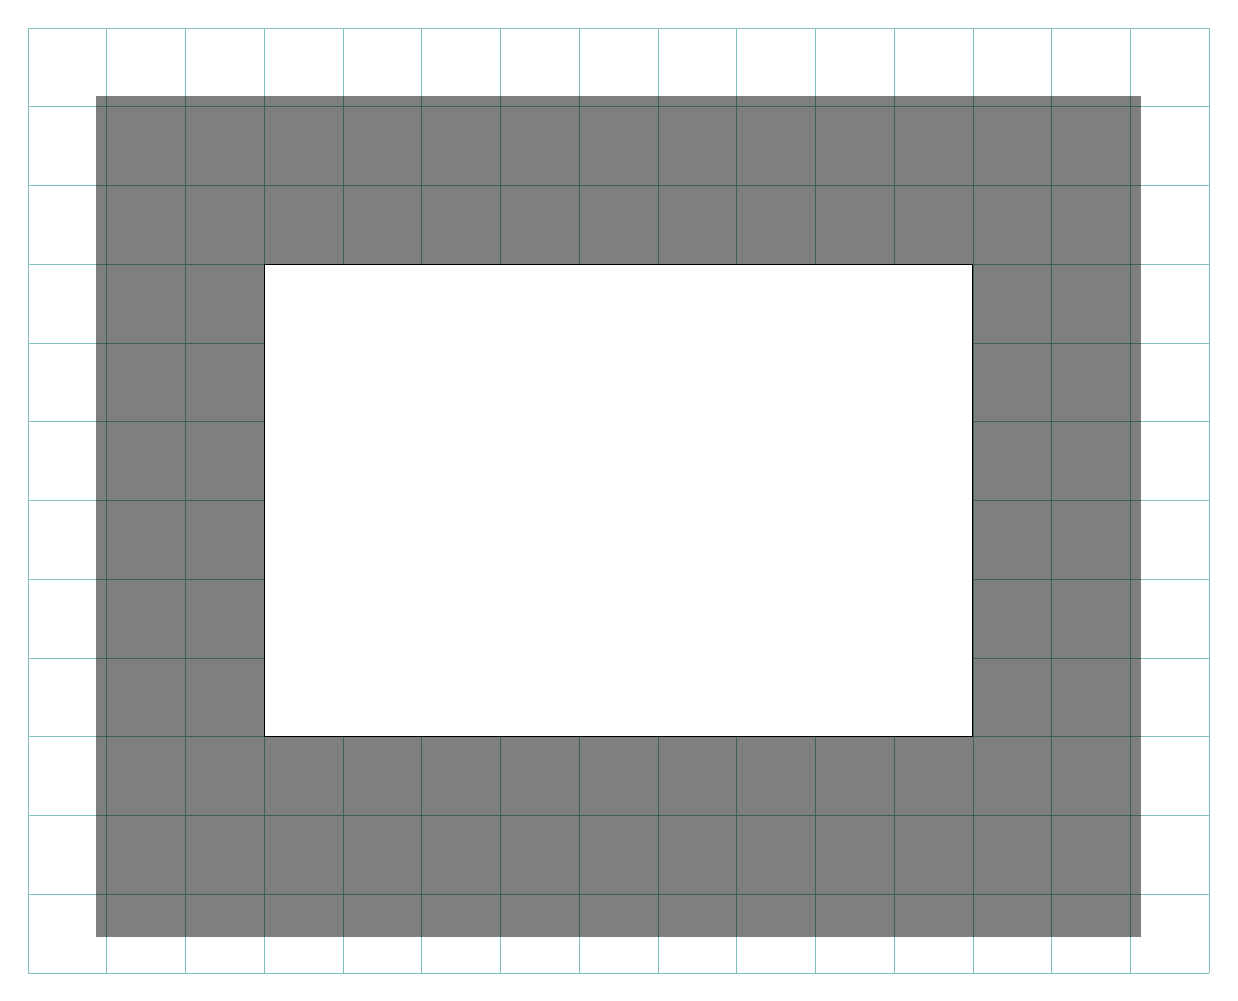
\begin{tikzpicture}
    \draw[help lines,very thin,color=blue!50!green!50,step=1] (-3.0, 3.0) grid +(15.0, -12.0);
    % Mat
    \draw[fill=black,opacity=0.5] (-2.1285,2.1285) rectangle +(13.257,-10.664);
    % Window
    \draw[fill=white] (0,0) rectangle +(9,-6);
\end{tikzpicture}
    \end{figure}



\end{document}